\chapter{Analisi}
\label{chap:analysis}
Il codec descritto, non è utiizzabile come versione stand-alone integrata in un software applicativo, ma potrà essere dispiegata come estensione chrome o browser alternativo in modo che sia fruibile sia da PC che da Smartphone e utilizzabile ogni qual volta viene scaricato un video con qualità almeno 720p. 
\section{Analisi Funzionale}
\label{sec:func}
Su questo tipo di analisi è necessario essere brevi, perché l'unica funzionalità offerta dall'encoder è appunto su richiesta dell'utente scaricare o visionare il video 720p o 1080p nel nostro formato H.265.
Le funzionalità descritte possono essere fruite nei seguenti modi:
\begin{itemize}
\item Installando come estensione browser il nostro progetto encoder e selezionando l'opzione "SI" al popup in apertura dopo il click del download.
\item Il nostro Codec verrà fornito nella lista delle risoluzioni di un video visionabile elencandolo come 720p e 1080p "ottimizzato", e verrà caricato alla scelta con la codifica in questione. 
\end{itemize}
Di seguito abbiamo previsto un'immagine utilizzata esclusivamente per documentare la metodologia del lavoro svolto di riconoscimento e segmentazione dei giocatori su un particolare frame:
\begin{figure}
   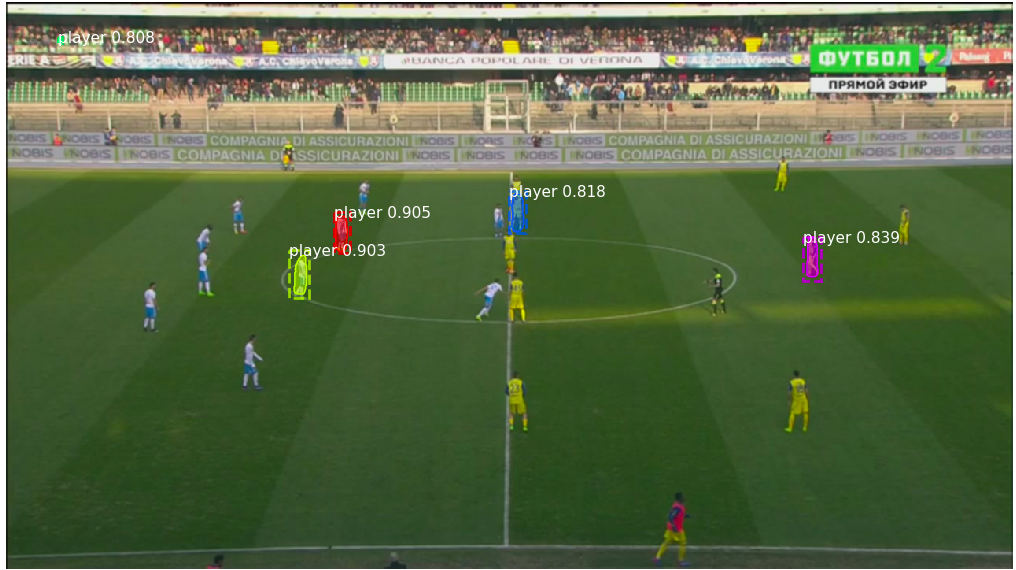
\includegraphics[width=\linewidth]{images/dim.png}
   \caption{dimostrazione di segmentazione giocatori}
   \label{fig:dim}
\end{figure}
\newpage
\section{Analisi Tecnica}
\label{sec:tech}
I file scritti personalmente che fanno parte di questo progetto sono 4 e ha anche una particolare importanza il file model.py non implementato personalmente, in quanto contiene la struttura di tutta la rete neurale da cui possiamo trarre i metodi per la creazione dell'oggetto che rappresenta la rete e per effettuare il training di essa.
\begin{itemize}
\item fine\_tuning.py
La classe è stata introdotta con la responsabilità di effettuare tutte le operazioni di training e di fine tuning della nostra rete e instanziare un oggetto soccer\_dataset su cui far partire due training: il primo sui top layers chiamati \emph{heads} e il secondo sui livelli \emph{4+} ovvero dallo strato 4 in su di una rete ResNet101. Questo è stato fatto attenendosi ad alcune fonti \textsuperscript{\cite{fine_tuning_book}}  e all'esempio \emph{balloon.py} poiché potevamo scegliere di fare un fine tuning sbloccando per l'allenamento anche solo i livelli più vicini agli heads: \emph{5+} oppure più lontani dagli heads: \emph{3+} o perfino allenare la rete totalmente.
\item soccer\_dataset.py
Carica un dataset di immagini di annotazioni in formato pascalVOC
\item main.py
Si occupa di gestire l'input della barra di comando che deve essere un video HD che mostra una partita di calcio, ne effettua l'instance segmentation, la quantizzazione e codifica per produrre un video Mp4 codificato H.265 con LPF.
\item clever\_config.py
Specifica la configurazione delle impostazioni di fine tuning desiderate che devono essere passate alla classe omonima per almeno i parametri fondamentali quali STEP\_PER\_EPOCH,GPU\_COUNT,NUM\_CLASSES oppure BATCH\_SIZE nel caso di parametro IMAGES\_PER\_GPU maggiore di 1.
\end{itemize}
Alla pagina seguente si riassume la struttura del progetto utilizzando un diagramma UML.

\subsection*{Main}
Come si può osservare dalla struttura del file main.py, questo non contiene una classe bensì un'istruzione che si accerta che il file main sia eseguito da riga di comando come primo file, e non sia quindi importato da altri files.
L'espressione che rende un booleano per confermare questa condizione è la seguente: \textbf{\_\_name\_\_ == "\_\_main\_\_"}
Come visibile dal diagramma UML collocato in seguito, il file main offre i seguenti metodi:
\begin{itemize}
\item Un metodo \emph{draw\_images\_with\_boxes} che si propone come metodo di "debug" in quanto serve solamente a mostrare il lavoro di riconoscimento e segmentazione svolto quando l'input è un'immagine, cosa che esula dai nostri obbiettivi di codifica \textbf{video}.
\item Un metodo \emph{is\_video\_file} che prende in ingresso un estensione e la confronta con tutte le esistenti estensioni video per capire se l'input in ingresso è effettivamente un video o meno.
\item Un metodo \emph{quantize\_frame} che è il metodo fulcro della nostra codifica per Region of Interest (RoI), infatti utilizza una copia del frame e vi applica un filtro passa-basso per rimuoverne le HF, dopodiché incolla le maschere dei giocatori del frame originale che le contiene ancora in HD sul frame copia, facendo risultare l'effetto LPF solo sulle regioni di non interesse.
\item Il metodo  \emph{main} che è il metodo contenente tutto il codice utile per arrivare ai seguenti risultati:
\begin{enumerate}
\item Ottenere i parametri inseriti a barra di comando
\item Controllare se c'è un parametro(booleano) fine tuning attivo e in caso affermativo delegare la responsabilità di effettuare il training alla classe omonima
\item Controllare se c'è un parametro input e in caso affermativo controllare se l'input è un video: in caso negativo se è un immagine la visualizza a video come instance segmentation
\item In caso che invece il parametro di input sia un video instanzia un oggetto \textbf{FFMpegWriter} con l'encoder \textbf{hevc} e con un coefficente di qualità costante adatto, dopodiché ne cicla i frame uno per uno
\item Una volta dentro il ciclo utiizza la funzione \emph{quantize\_frame} per applicare un LPF al frame corrente, dopodiché lo scrive nel nuovo video con la funzione \emph{write} di \textbf{FFMpegWriter}
\item Alla fine del ciclo, tutti i frame sono stati scritti in modo codificato "2 volte", ovvero una grazie all'oggetto \textbf{FFMpegWriter} che ha tolto una quantità di informazioni trascurabile e l'altra grazie al nostro LPF. Infine quindi le risorse vengono rilasciate e il nuovo video viene salvato con estensione contenitore generica .mp4
\end{enumerate}
\end{itemize}
\subsection*{Classe model}
La descrizione di ciò che le classi operano è riassunta nel preambolo di questa sezione, essendo esse strettamente collegate ai rispettivi files in python. Descriviamo ora in particolare la classe non implementata da noi denominata \emph{model} che chiameremo con il suo alias \emph{modellib} e il suo utilizzo, dopodiché ci soffermiamo su attributi e metodi delle classi corrispondenti ai files già descritti in precedenza.
Come visibile dal diagramma UML collocato in seguito, la classe modellib all'interno di model.py deve offrire:
\begin{itemize}
\item Un attributo accessibile dal model che rappresenta i pesi\emph{(weights)} allenati della rete, accessibile come keras\_model.history.history
\item Un costruttore statico utilizzabile con l'istruzione modellib.MaskRCNN che restituisce un'istanza del model.
\item Un metodo che viene usato per caricare i \emph{weights} escludendo i 4 layers che comprendono la lista di tutte le labels su cui è stata allenata originariamente la rete MaskRCNN, in modo da personalizzare il training su esclusivamente i giocatori e la palla, denominato \emph{load\_weights.}
\item Un metodo denominato \emph{train} che consente effettivamente di effettuare il training dei \emph{weights} specificando il training set e il test set, i layers bersaglio che devono essere sbloccati per il fine tuning(heads o 3/4/5+),il numero di epochs e il learning rate che vengono ricavati dal file clever\_config.py per best practice e le trasformazioni casuali sui frames (\emph{augmentation}) per un allenamento dinamico.
\item Un metodo denominato \emph{save\_weigths} che viene utilizzato per salvare sul file system i \emph{weights} addestrati dopo il fine tuning e viene richiamato con keras\_model.save\_weigths.
\end{itemize}

\subsection*{Classe SoccerDataset}
La classe SoccerDataset ridefinisce i metodi della sua superclasse Dataset,eccetto un metodo che merita una menzione particolare chiamato \emph{prepare}, che presa per scontata l'equivalenza tra labels e classi,offre le seguenti operazioni:
\begin{itemize}
\item Il metodo suddetto  salva tutte le informazioni delle classi come il numero e il nome di esse, compresi gli IDs in forma autoincrementante dalla variabile \emph{self.class\_info}
\item Mappa IDs interni(class e images) partendo dalle info come \emph{self.class\_info} e \emph{self.class\_ids}
\item Mappa i sorgenti(sources) verso i class\_ids che essi supportano.
\end{itemize}
Il metodo che è sottoposto a ovveride nella classe figlia chiamato \emph{load\_dataset}, come si può osservare dal nome autodocumentante, si limita a caricare le classi del dataset personalizzato.
Gli altri metodi, che non sono sottoposti a override ma sono totalmente nuovi nella classe figlia SoccerDataset, sono elencati seguentemente con i loro effetti:
\begin{itemize}
\item extract\_polygons : è il metodo fondamentale per la lettura delle annotazioni JSON di un immagine scelta che contengono le informazioni sui poligoni che descrivono i giocatori e la decodifica dei dati su di essi per poi essere salvati in un array di polygons che sarà restituito al chiamante insieme alla larghezza e all'altezza dell'immagine.
\item load\_mask : il metodo corrente, data un'ID intera di un'immagine, restituisce la sua altezza,larghezza e l'array di poligoni che sono stati estratti con il metodo \emph{extract\_polygons}
\item image\_reference : ritorna la path del'immagine 
\end{itemize}

\subsection*{Classe FineTuning}
La classe sunnomminata si dedica innanzitutto a creare una configurazione personalizzata CleverConfig che sarà utilizzata nella stessa classe come parametro per costruttore del model, nell'unico metodo esistente che è:
\begin{itemize}
\item start: questo metodo si dedica alla creazione dei train\_set e test\_set per l'allenamento della rete, alla creazione dell'oggetto model per il caricamento dei pesi e per il loro allenamento in 2 fasi: prima quello degli \emph{heads} e successivamente quello dei livelli \emph{4+}
\end{itemize}
\subsection*{Classe CleverConfig}
Effettua l'ovverride della classe Config standard che è anonima ma contiene tutti i parametri per effettuare un fine tuning o training da una rete blackbox, ovvero che non ha ricevuto nessun addestramento.\\
I parametri con cui la classe Config se non ridefinita performerebbe il training della rete sono i seguenti(trascritti direttamente dalla classe config.py):\\

\begin{lstlisting}
class Config(object):

 
    NAME = None  # Override in sub-classes

    GPU_COUNT = 1

  
    IMAGES_PER_GPU = 2

    STEPS_PER_EPOCH = 1000

  
    VALIDATION_STEPS = 50

    BACKBONE = "resnet101"

    COMPUTE_BACKBONE_SHAPE = None

    # The strides of each layer of the FPN Pyramid. These values
    # are based on a Resnet101 backbone.
    BACKBONE_STRIDES = [4, 8, 16, 32, 64]

    # Size of the fully-connected layers in the classification graph
    FPN_CLASSIF_FC_LAYERS_SIZE = 1024

    # Size of the top-down layers used to build the feature pyramid
    TOP_DOWN_PYRAMID_SIZE = 256

    # Number of classification classes (including background)
    NUM_CLASSES = 1  # Override in sub-classes

    # Length of square anchor side in pixels
    RPN_ANCHOR_SCALES = (32, 64, 128, 256, 512)

    # Ratios of anchors at each cell (width/height)
    # A value of 1 represents a square anchor, and 0.5 is a wide anchor
    RPN_ANCHOR_RATIOS = [0.5, 1, 2]

    # If 1 then anchors are created for each cell in the backbone feature map.
    # If 2, then anchors are created for every other cell, and so on.
    RPN_ANCHOR_STRIDE = 1

    # Non-max suppression threshold to filter RPN proposals.
    # You can increase this during training to generate more propsals.
    RPN_NMS_THRESHOLD = 0.7

    # How many anchors per image to use for RPN training
    RPN_TRAIN_ANCHORS_PER_IMAGE = 256
    
    # ROIs kept after tf.nn.top_k and before non-maximum suppression
    PRE_NMS_LIMIT = 6000

    # ROIs kept after non-maximum suppression (training and inference)
    POST_NMS_ROIS_TRAINING = 2000
    POST_NMS_ROIS_INFERENCE = 1000

    # If enabled, resizes instance masks to a smaller size to reduce
    # memory load. Recommended when using high-resolution images.
    USE_MINI_MASK = True
    MINI_MASK_SHAPE = (56, 56)  # (height, width) of the mini-mask

    IMAGE_RESIZE_MODE = "square"
    IMAGE_MIN_DIM = 800
    IMAGE_MAX_DIM = 1024
  
    IMAGE_MIN_SCALE = 0
       IMAGE_CHANNEL_COUNT = 3

    # Image mean (RGB)
    MEAN_PIXEL = np.array([123.7, 116.8, 103.9])

       TRAIN_ROIS_PER_IMAGE = 200

    # Percent of positive ROIs used to train classifier/mask heads
    ROI_POSITIVE_RATIO = 0.33

    # Pooled ROIs
    POOL_SIZE = 7
    MASK_POOL_SIZE = 14

    # Shape of output mask
    # To change this you also need to change the neural network mask branch
    MASK_SHAPE = [28, 28]

    # Maximum number of ground truth instances to use in one image
    MAX_GT_INSTANCES = 100

    # Bounding box refinement standard deviation for RPN and final detections.
    RPN_BBOX_STD_DEV = np.array([0.1, 0.1, 0.2, 0.2])
    BBOX_STD_DEV = np.array([0.1, 0.1, 0.2, 0.2])

    # Max number of final detections
    DETECTION_MAX_INSTANCES = 100

    DETECTION_MIN_CONFIDENCE = 0.7

    # Non-maximum suppression threshold for detection
    DETECTION_NMS_THRESHOLD = 0.3

  
    LEARNING_RATE = 0.001
    LEARNING_MOMENTUM = 0.9

    # Weight decay regularization
    WEIGHT_DECAY = 0.0001

    LOSS_WEIGHTS = {
        "rpn_class_loss": 1.,
        "rpn_bbox_loss": 1.,
        "mrcnn_class_loss": 1.,
        "mrcnn_bbox_loss": 1.,
        "mrcnn_mask_loss": 1.
    }
    
    USE_RPN_ROIS = True

    TRAIN_BN = False  # Defaulting to False since batch size is often small

    # Gradient norm clipping
    GRADIENT_CLIP_NORM = 5.0
\end{lstlisting}

Per effettuare quindi un fine tuning addatto all'evenienza abbiamo ridefinito i seguenti parametri, con il nostro ovveride della classe Config:
\begin{lstlisting}
class CleverConfig(Config):
    # give the configuration a recognizable name
    NAME = "clever_coding_config"

    # set the number of GPUs to use along with the number of images
    # per GPU
    GPU_COUNT = 1
    IMAGES_PER_GPU = 1
    # Skip detections with < 90% confidence
    DETECTION_MIN_CONFIDENCE = 0.8
    # batch_size=2. Samples=50. steps=50/2
    STEPS_PER_EPOCH = 120
    VALIDATION_STEPS = 25
    BATCH_SIZE = 1 #GPU_COUNT*IMAGES_PER_GPU
    # number of classes (we would normally add +1 for the background
    # but the background class is *already* included in the class
    # names)
    NUM_CLASSES = 1 + 2

\end{lstlisting}
\newpage
\begin{sidewaysfigure}
   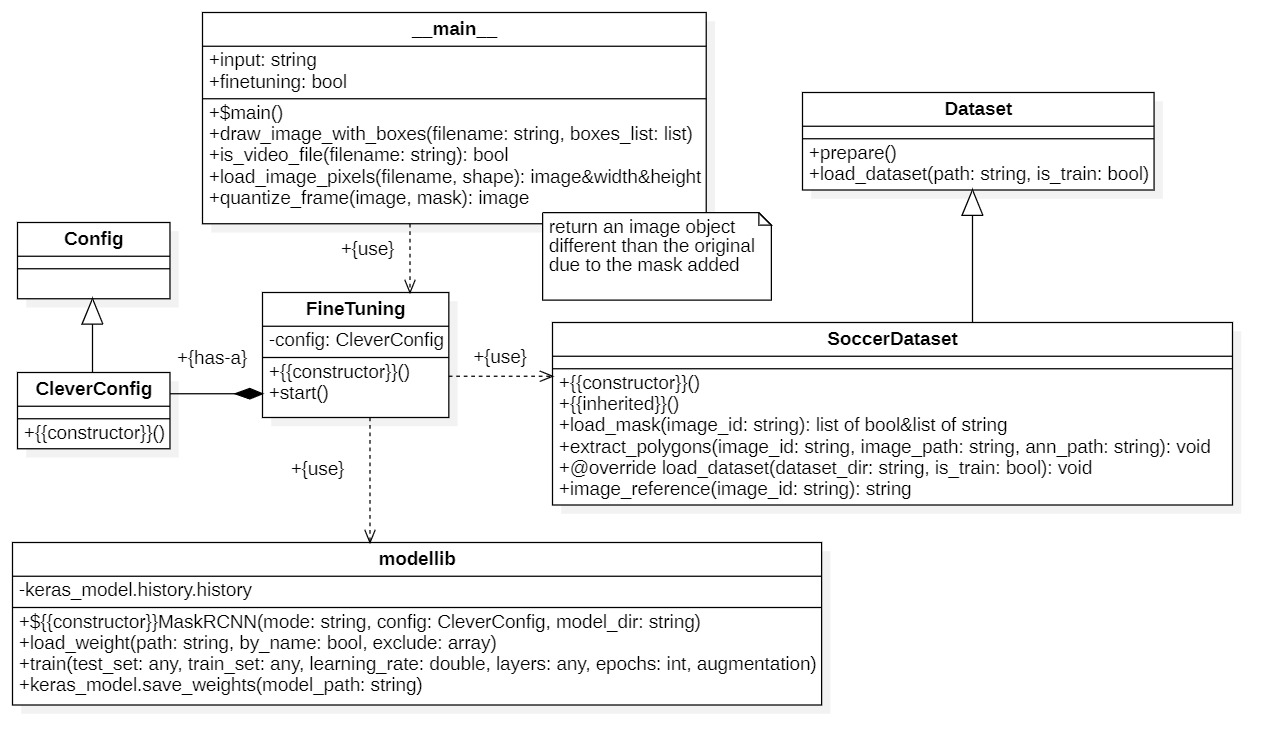
\includegraphics[width=\linewidth]{images/UML.jpg}
    \caption{Diagramma UML del progetto}
    \label{fig:uml}
\end{sidewaysfigure}






